%=============================================================================
\section{Robustness and Scope}
\label{sec:robustness}
%=============================================================================

Section~\ref{sec:results} establishes an advantage under one annotation, in one
catalogue, at one operating point. This section attacks each of those in turn,
in that order.

The first three subsections concern the annotation, which is the assumption the
paper most depends on and the one a reader is most entitled to distrust: we
report the result across a distribution over the assumed values, then remove
the assumed values entirely by learning them from logs, then show which routes
to the same parameter do \emph{not} work and why. The next two concern the
operating point---how noisy users must be, and how wrong the annotation may
be---and the two after that concern the catalogue, establishing the scope
condition under which any of this transfers. The last two return to the
observation model itself and relax its two structural assumptions.

\subsection{Robustness to the Assumed Crossover Values}
\label{sec:results-ensemble}

The three numbers $(0.03, 0.15, 0.30)$ are assumed, not measured. The
strongest objection to this work is therefore that its headline result could be
an artefact of having picked them. We answer it by refusing to pick.

The design is stated in Section~\ref{sec:priors} and matters more than the
outcome. The \emph{deployed} system is held fixed: RAIG-tiered always assumes
the point values, because that is what a practitioner who followed this paper
would actually ship. What varies is the \emph{truth}. For each of $60$ draws we
sample a per-attribute true crossover from the tier priors---scaled Beta
distributions on $[0,\tfrac12)$ with the point values as means and
deliberately low concentration---and run the fixed system against that world.
Because the draw is per attribute, every world contains within-tier
heterogeneity that the three-tier specification structurally cannot represent,
and because the semi-objective and subjective priors overlap
($[0.037, 0.300]$ against $[0.142, 0.437]$), many worlds locally violate the
tier ordering the system assumes. The question is not whether the method works
when it knows the answer. It is whether a system built on three guessed numbers
still beats current practice when the world does not match those numbers.

It does, in every draw. Across $60$ worlds the mean paired advantage of
RAIG-tiered over IG+soft-uniform is $+6.21\pp$, with median $+5.33\pp$ and a
$95\%$ range across worlds of $[+1.33, +13.02]\pp$. The advantage is positive
in $100\%$ of draws; its minimum over all $60$ is $+1.33\pp$. Each draw is only
$n=150$ trials, so individual draws are underpowered, yet $53\%$ of them reach
exact-McNemar significance at $\alpha = 0.05$ on their own, and \emph{no} draw
produces a significant win for classical information gain.

Two further readings are worth recording. First, the advantage does not depend
on the drawn world being an easy one: the correlation between the paired
advantage and the mean true crossover of the drawn world is $-0.18$, so if
anything the method does slightly better in the less noisy worlds, and it never
depends on a favourable draw. Second, the gap to the oracle is real and
quantified: mean accuracy across the ensemble is $2.58\%$ for IG+soft-uniform,
$8.79\%$ for RAIG-tiered and $11.84\%$ for RAIG-oracle. Three coarse tiers
recover about $72\%$ of what perfect per-attribute knowledge would buy---which
is the answer to ``how much would measuring $\varepsilon$ properly be worth'',
and it is a meaningful amount but not a transformative one.

This experiment does not remove the need for the user study of
Appendix~\ref{app:protocol}. It changes what that study is for: not to
establish whether the correction works, but to reduce the residual $28\%$.

\subsection{Removing the Assumption: a Crossover Vector Learned from Logs}
\label{sec:results-em}

Section~\ref{sec:results-ensemble} shows the conclusion survives the tier values
being wrong. This subsection removes them.

We deploy the incumbent---classical information gain at a single global
crossover, the system a practitioner already has---for $600$ sessions of $T=20$
under the heterogeneous $\lambda=1.0$ channel, log the questions asked and the
answers received, and run the EM of Section~\ref{sec:reliability-em} for eight
iterations from a neutral start of $\hat\varepsilon = 0.10$ for every attribute.
The estimator is given no annotation, no tier structure, no labels, and no
knowledge of any session's target. It is then evaluated exactly like every other
specification, under the primary protocol.

\begin{table}[t]
\caption{A crossover vector learned from $600$ logged sessions, with nothing
assumed. ``Explore'' is the fraction of logged questions asked uniformly at
random rather than greedily. $\rho$ and MAE compare the learned vector with the
true one across the $20$ non-degenerate attributes, and are diagnostics only:
the estimator never sees either. Accuracies are the primary protocol,
heterogeneous $\lambda = 1.0$, $n = 900$.}
\label{tab:em}
\centering
\scriptsize
\begin{tabular}{@{}rrrrrrr@{}}
\toprule
\textbf{explore} & \textbf{min obs} & \textbf{$\rho$} & \textbf{MAE} &
\textbf{IG} & \textbf{RAIG-EM} & \textbf{RAIG-tiered} \\
\midrule
0.00 & 6  & $+0.829$ & 0.054 & 3.22 & 8.33 & 8.33 \\
0.10 & 26 & $+0.709$ & 0.066 & 3.22 & 8.22 & 8.33 \\
0.25 & 34 & $+0.806$ & 0.057 & 3.22 & 7.78 & 8.33 \\
\bottomrule
\end{tabular}
\end{table}

\emph{The learned vector is as good as the annotation.} With no exploration at
all, RAIG-EM reaches $8.33\%$ against the incumbent's $3.22\%$
($+5.11\pp$, exact McNemar $p = 2.3\times10^{-7}$), and against RAIG-tiered it
is a dead heat: $38$ discordant pairs in each direction, $p = 1.00$. Three
curator-assigned constants and a vector inferred from six hundred sessions of
ordinary use produce the same accuracy. The three numbers this paper assumed can
therefore be replaced, in a deployed system, by numbers the system measures for
itself.

\emph{The estimate is attenuated, and it does not matter.} The learned vector
recovers the ordering well ($\rho = +0.829$, MAE $0.054$) but compresses the
range, and it does so systematically: subjective attributes whose true crossover
is $0.300$ are estimated between $0.158$ and $0.230$, while objective attributes
at $0.030$ are estimated between $0.005$ and $0.085$. The compression is
expected. The posterior used in \eqref{eq:em-disagree} is itself diffuse---the
incumbent identifies the target only $3.22\%$ of the time---so the expected
disagreement at each turn is pulled towards the split mass, which regresses
every estimate towards the middle. That this costs nothing is
Proposition~\ref{prop:uniform} at work: selection depends on the ordering of
$\hat\varepsilon$ across attributes, and a monotone attenuation preserves it.
An estimator that is reliably ordered and badly calibrated is exactly what this
acquisition function needs.

\emph{Exploration is unnecessary here, which we did not expect.} A greedy
incumbent asks its least-favoured attribute only six times in six hundred
sessions, and we anticipated that the estimates for those attributes would be
too noisy to use. Forcing coverage by asking a fraction of questions at random
raises the minimum observation count from $6$ to $34$ and does not help:
accuracy goes from $8.33\%$ at no exploration to $8.22\%$ at $10\%$ and $7.78\%$
at $25\%$, neither significantly different from the tiered specification
($p = 1.00$ and $p = 0.68$). The reason is visible once stated. An attribute the
greedy selector never asks is an attribute whose $\hat\varepsilon$ barely
affects the ranking of the questions it does ask, so estimating it badly costs
little; and the turns spent exploring are turns not spent identifying, which
degrades the very posteriors the M-step depends on. A practitioner should
collect logs from the system they already run, and not pay for randomisation.

\emph{What this does and does not remove.} It removes the objection that the
headline result depends on three invented numbers: it does not, and the same
result is available to a practitioner with no curator and no annotation, at the
cost of running the incumbent first. It does not remove the need for the user
study of Appendix~\ref{app:protocol}, for a reason worth stating plainly. Our
logs are generated by a simulator whose users err at rates drawn from the tier
annotation, so what EM recovers is the structure we put in. The experiment
establishes that the estimator is \emph{identifiable and sufficient}---that this
much can be recovered from logs of this size without labels, and that recovering
it is enough to match the annotation---and not that real users' errors have this
form. That remains the open question, and it is the same one throughout.

\subsection{What Cannot Be Derived from the Catalogue Alone}
\label{sec:results-psycho}

The learned vector of the previous subsection needs a deployed system to
generate logs. Before there is one, is there a specification that needs neither
logs nor a curator? Section~\ref{sec:psychophysical} supplies the obvious
candidate, and this subsection reports that it does not work and exactly why,
because the failure delimits the contribution more sharply than the success
does.

\emph{The candidate.} Every attribute derived by cutting a continuous column
has boundaries, and where those boundaries fall is a property of the data. We
recover the cut points the original pipeline used---the shipped columns are
threshold cuts, not quantile bins, and the recovered boundaries reproduce the
shipped labels for $99.5\%$ of items or better on all ten attributes---place a
listener's perception at $\sigma$ z-scored standard deviations from the truth,
and compute the probability that the reported label changes. This yields
$\hat\varepsilon_f$ for the ten binned attributes with no annotation at all.
The remaining eleven attributes have no continuous source, so they take a
single constant $\varepsilon_{\text{cat}}$. Two assumed scalars replace three
assumed tier values, and the shape across the binned attributes comes entirely
from the data.

\emph{It fails, at every setting we tried} (Table~\ref{tab:psycho}). The best
cell reaches $4.33\%$ ($\sigma = 0.10$, $\varepsilon_{\text{cat}} = 0.10$)
against the tiered specification's $8.33\%$ and the incumbent's $3.22\%$. All
nine cells are significantly worse than the tiered annotation, by between
$4.00$ and $7.56$ percentage points; not one is significantly better than
classical information gain, and three are significantly worse than it.

\begin{table}[t]
\caption{The catalogue-derived specification, swept over its two parameters:
perceptual noise $\sigma$ and the constant $\varepsilon_{\text{cat}}$ given to
the eleven attributes with no continuous source. Top-1 accuracy (\%), primary
condition, $n = 900$. The incumbent scores $3.22$ and the tiered specification
$8.33$ in every row. No setting of the two parameters recovers the annotation.}
\label{tab:psycho}
\centering
\footnotesize
\begin{tabular}{@{}rrrrr@{}}
\toprule
$\sigma$ & $\varepsilon_{\text{cat}}$ & \textbf{RAIG-psycho} &
\textbf{vs IG} & \textbf{vs tiered} \\
\midrule
0.10 & 0.01 & 3.33 & $+0.11$ & $-5.00$ \\
0.10 & 0.03 & 1.89 & $-1.33$ & $-6.44$ \\
0.10 & 0.10 & 4.33 & $+1.11$ & $-4.00$ \\
0.25 & 0.01 & 2.89 & $-0.33$ & $-5.44$ \\
0.25 & 0.03 & 2.44 & $-0.78$ & $-5.89$ \\
0.25 & 0.10 & 2.78 & $-0.44$ & $-5.56$ \\
0.50 & 0.01 & 1.89 & $-1.33$ & $-6.44$ \\
0.50 & 0.03 & 1.00 & $-2.22$ & $-7.33$ \\
0.50 & 0.10 & 0.78 & $-2.44$ & $-7.56$ \\
\bottomrule
\end{tabular}
\end{table}

\emph{The reason is structural, not a tuning failure.} The eleven attributes
without a continuous source are not a homogeneous group. Six are the objective
metadata---genre, language, content rating, artist type, release type, track
version---which a listener answers almost perfectly. The other five are mood,
tempo, key, mode and time signature, which a non-musician answers close to
chance. A specification that assigns one constant to all eleven must place
these two groups at the same crossover, and no choice of that constant can be
right for both: raising it to describe key and mode makes the system distrust
language and genre, which are its most reliable questions. That is visible in
the sweep, where increasing $\varepsilon_{\text{cat}}$ from $0.01$ to $0.10$
helps at $\sigma = 0.10$ and hurts at $\sigma = 0.50$, with no setting escaping
the bind.

What separates those two groups is not a boundary effect that a psychophysical
model could capture. It is knowledge: a listener does not fail to name the key
of a song because the boundary between keys is fuzzy, but because they never
learned to name keys. The taxonomy this paper's annotation encodes---objective,
semi-objective, subjective---is doing work that no measurement on the catalogue
can do, because the difficulty is a fact about people rather than about the
data. Section~\ref{sec:results-em} is the resolution: EM over interaction logs
recovers exactly this distinction, because logs are observations of people.

We therefore report three routes to $\hat{\boldsymbol\varepsilon}$ and one
dead end. A curator's three tiers work. A vector learned from logs works and
needs no curator. Repeated-item discordance (Section~\ref{sec:results-main})
and the psychophysical model here both fail, and they fail the same way: each
measures a property of the catalogue, and answerability is a property of the
people using it.

\subsection{How Noisy Must Users Be Before the Correction Pays?}
\label{sec:results-lambda}

Table~\ref{tab:main} reports three noise multipliers and shows RAIG-tiered
trailing at $\lambda \le 0.5$ and leading at $\lambda \ge 1.0$. That leaves the
crossing unlocated, and the crossing is the number a practitioner actually
needs: it says how unreliable your users have to be before the correction is
worth making. Table~\ref{tab:lambda} sweeps a finer grid.

\begin{table}[t]
\caption{Top-1 accuracy (\%) against the noise multiplier $\lambda$, which
scales the tiered crossover values without changing their structure;
$\bar\varepsilon$ is the resulting catalogue-average crossover. $\Delta$ is
RAIG-tiered minus IG+soft-uniform, $n = 450$ paired trials per row, and $p$ is
the exact McNemar $p$-value. The advantage changes sign between
$\lambda = 0.5$ and $\lambda = 0.625$.}
\label{tab:lambda}
\centering
\scriptsize
\begin{tabular}{@{}rrrrrrr@{}}
\toprule
$\lambda$ & $\bar\varepsilon$ & \textbf{IG+soft-u.} & \textbf{Learned} &
\textbf{RAIG-tier.} & \textbf{$\Delta$ (pp)} & \textbf{$p$} \\
\midrule
0.000 & 0.000 & 96.0 & 91.1 & 42.4 & $-53.6$ & $6{\cdot}10^{-73}$ \\
0.250 & 0.025 & 50.9 & 43.1 & 28.4 & $-22.4$ & $6{\cdot}10^{-14}$ \\
0.500 & 0.049 & 24.0 & 19.1 & 19.6 & $-4.4$  & $0.088$ \\
0.625 & 0.061 & 14.2 & 12.0 & 16.2 & $+2.0$  & $0.407$ \\
0.750 & 0.074 & 7.1  & 7.1  & 12.9 & $+5.8$  & $0.0026$ \\
0.875 & 0.086 & 4.2  & 4.7  & 10.9 & $+6.7$  & $0.0001$ \\
1.000 & 0.098 & 2.4  & 1.8  & 7.8  & $+5.3$  & $0.0002$ \\
1.250 & 0.123 & 0.9  & 0.2  & 4.2  & $+3.3$  & $0.0015$ \\
1.500 & 0.147 & 0.2  & 0.2  & 3.6  & $+3.3$  & $0.0003$ \\
2.000 & 0.196 & 0.0  & 0.0  & 2.0  & $+2.0$  & $0.0039$ \\
\bottomrule
\end{tabular}
\end{table}

Linear interpolation of the paired difference places the crossing at
$\lambda = 0.586$, which corresponds to a catalogue-average crossover of
$0.0575$---tier values of $(0.018, 0.088, 0.176)$ rather than
$(0.03, 0.15, 0.30)$. The practitioner-facing statement is therefore: once
users get roughly one answer in seventeen wrong on average, and that error is
distributed across attributes the way the annotation says, correcting the
acquisition function begins to pay. Below that, do not.

Two features of the sweep deserve comment. The advantage is not monotone in
$\lambda$: it peaks at $+6.7\pp$ around $\lambda = 0.875$ and then declines,
because at high noise every method is being pushed towards the floor and there
is less accuracy left to win. And the deficit at $\lambda = 0$ is enormous
($-53.6\pp$), which is the clean-condition collapse of
Section~\ref{sec:results-main} seen as a limit rather than as an anomaly:
reliability weighting is a correction for a channel, and applying it to a
noiseless channel is not conservative, it is actively harmful. The learned
policy tracks classical information gain across the entire sweep, never
crossing above it except by noise, which is the same conclusion
Section~\ref{sec:results-learned} reaches at a single operating point.

\subsection{How Wrong May the Annotation Be?}
\label{sec:results-corruption}

Section~\ref{sec:results-ensemble} varies the tier \emph{values} while keeping
each attribute in its correct tier. The complementary failure is a curator who
puts attributes in the wrong tier, and it is the more likely one in practice:
guessing that subjective attributes are around $0.3$ is easier than deciding
whether loudness is semi-objective or subjective. We therefore mis-tier a
fraction $\phi$ of attributes, drawn at random and reassigned to a different
tier, and sweep $\phi$ from $0$ to $1$ with the truth held fixed, so the only
thing degrading is the annotation (Table~\ref{tab:corruption}).

This replaces a misspecification surface that could not have shown anything.
Sweeping a \emph{homogeneous} assumed crossover against a homogeneous true one,
as one might naturally do, cannot affect selection at all: by
Proposition~\ref{prop:uniform} a constant $\hat\varepsilon$ adds the same
capacity term to every question and leaves the ranking exactly unchanged, so
such a grid measures only the belief update. The axis that bears on selection
is whether attributes are in the right tier.

\begin{table}[t]
\caption{Degrading the tier annotation. $\phi$ is the fraction of the $21$
attributes reassigned to a different tier; the truth is held fixed at
heterogeneous $\lambda = 1.0$. $\Delta$ is RAIG minus IG+soft-uniform, averaged
over three independent corruptions ($\phi = 0$ is deterministic, hence one),
each at $n = 300$ paired trials; the range is over those corruptions. The
spread is wide because $n = 300$ at these accuracies yields only a handful of
successes---read the trend, not the individual rows.}
\label{tab:corruption}
\centering
\footnotesize
\begin{tabular}{@{}rrrrr@{}}
\toprule
$\phi$ & \textbf{mis-tiered} & \textbf{IG+soft-u.} & \textbf{RAIG} &
\textbf{$\Delta$ (pp)} \\
\midrule
0.0 & 0  & 1.67 & 6.00 & $+4.33$ \\
0.1 & 2  & 1.67 & 5.44 & $+3.78$ \\
0.2 & 4  & 1.67 & 4.56 & $+2.89$ \\
0.3 & 6  & 1.67 & 4.00 & $+2.33$ \\
0.4 & 8  & 1.67 & 2.89 & $+1.22$ \\
0.5 & 10 & 1.67 & 4.22 & $+2.56$ \\
0.6 & 13 & 1.67 & 2.33 & $+0.67$ \\
0.8 & 17 & 1.67 & 1.22 & $-0.44$ \\
1.0 & 21 & 1.67 & 1.11 & $-0.56$ \\
\bottomrule
\end{tabular}
\end{table}

The advantage decays roughly linearly and changes sign between $\phi = 0.6$ and
$\phi = 0.8$; linear interpolation puts the break-even at $\phi = 0.72$. Taken
at face value that says the curator may mis-tier about fifteen of the
twenty-one attributes before the correction stops paying, which is a
remarkable amount of slack. We would not defend the second digit. At $n = 300$
and accuracies in the low single digits each cell rests on a handful of correct
identifications, the spread across independent corruptions at a fixed $\phi$ is
of the same order as the effect being measured---at $\phi = 0.5$ the three
corruptions give $+1.00$, $+4.33$ and $+2.33$, which is why that row sits above
its neighbours---and the honest reading is that the break-even lies somewhere
between $\phi = 0.6$ and $\phi = 0.8$ rather than at any particular point in
between.

The qualitative conclusion survives that caveat, and it is the one that matters
for deployment: the annotation is not a precision instrument. Getting a
\emph{majority} of attributes into the right tier is sufficient, and the method
degrades gracefully rather than falling off a cliff. Even at $\phi = 1$, where
every attribute has been moved, RAIG loses by only $0.56\pp$---because
reassignment is to one of the two other tiers rather than to an adversarial
one, so some of the objective/subjective contrast survives by chance. The
adversarial column of Table~\ref{tab:main}, where the assignment is inverted
rather than scrambled, is the genuinely damaging case, and it costs
$13.45\pp$.

\subsection{Other Domains: the Bias Is Absent, the Benefit Is Not}
\label{sec:results-domains}

The bias characterised in Section~\ref{sec:results-bias} does not replicate in
the two non-music catalogues, and we report that plainly because it is a
confirmation of the mechanism rather than a failure of the result.

On mushroom, the Kruskal--Wallis test across tiers gives $H = 1.75$
($p = 0.416$) and Kendall's $\tau_b$ is $+0.006$ ($p = 0.974$): no relationship
whatsoever, with tier means of $0.780$, $0.976$ and $0.803$ bits. On
dermatology the omnibus test is marginal ($H = 6.21$,
$p = 0.045$) but the rank correlation is \emph{positive}, $\tau_b = +0.135$
($p = 0.335$), and the tier means are non-monotone---$0.797$, $0.969$, $0.762$
bits for objective, semi-objective and subjective---so the effect there is that
the middle tier splits best, which is not the pattern the bias predicts and
does not favour our method. Neither catalogue contains a continuous attribute
to discretise, and the mechanism we blame is discretisation acting on
perceptual quantities. Predicting the absence of an effect and then observing
it is stronger evidence for the mechanism than a third positive replication
would have been.

What happens next is the interesting part, and it was not predicted
(Table~\ref{tab:domains}).

\begin{table}[t]
\caption{Cross-domain comparison, top-1 accuracy (\%) at $T=20$, $n=600$
paired trials per cell. The bias is present only in music, yet
reliability-aware selection is inert on mushroom and transformative on
dermatology. The last row gives the exact McNemar $p$-value for RAIG-tiered
against IG+soft-uniform in that column.}
\label{tab:domains}
\centering
\scriptsize
\begin{tabular}{@{}lrrrrrr@{}}
\toprule
& \multicolumn{3}{c}{\textbf{Mushroom}} & \multicolumn{3}{c}{\textbf{Dermatology}} \\
\cmidrule(lr){2-4}\cmidrule(lr){5-7}
\textbf{Method} & $\lambda{=}0.5$ & $1.0$ & $1.5$ & $\lambda{=}0.5$ & $1.0$ & $1.5$ \\
\midrule
Random+soft       & 0.3  & 0.2  & 0.0 & 26.2 & 9.7  & 3.0  \\
IG+hard           & 27.7 & 8.0  & 1.0 & 47.0 & 20.0 & 7.8  \\
IG+soft-uniform   & 31.7 & 10.5 & 2.3 & 84.5 & 34.7 & 6.0  \\
IG+soft-objective & 1.7  & 1.2  & 0.8 & 18.5 & 17.3 & 15.8 \\
RAIG-tiered       & 31.5 & 10.3 & 2.7 & 92.7 & 73.0 & 48.3 \\
RAIG-oracle       & 35.7 & 10.3 & 3.8 & 94.5 & 73.0 & 46.3 \\
\midrule
McNemar $p$ & $1.00$ & $1.00$ & $0.85$ &
  $6{\cdot}10^{-7}$ & $3{\cdot}10^{-52}$ & $5{\cdot}10^{-71}$ \\
\bottomrule
\end{tabular}
\end{table}

On mushroom, reliability-aware selection changes nothing: $10.3\%$ against
$10.5\%$ at $\lambda = 1.0$, McNemar $p = 1.00$. On dermatology it more than
doubles accuracy, $73.0\%$ against $34.7\%$, and the effect grows as users get
noisier. Two catalogues with no measurable bias, and diametrically opposite
outcomes. The correlation between informativeness and reliability evidently is
not what decides whether the correction pays, and the next subsection
identifies what does.

\subsection{When Reliability-Aware Selection Pays}
\label{sec:results-synthetic}

Two properties of a catalogue matter, and they are separate.

\emph{Correlation determines whether classical information gain is actively
harmed.} In music, the selector seeks out unreliable questions: it asks at mean
true crossover $0.225$ against a catalogue average of $0.098$
(Table~\ref{tab:asked}). In dermatology it does not: it asks at $0.236$ against
a catalogue average of $0.240$, which is to say it is behaving no worse than
chance with respect to reliability. In mushroom it is mildly \emph{better} than
chance, asking at $0.170$ against an average of $0.197$. This is exactly the
ordering the bias measurement predicts, and it confirms that the bias
measurement is measuring what we say it does.

\emph{Heterogeneity, plus the availability of reliable information, determines
whether reliability-aware selection can gain.} Even when classical information
gain is not being actively misled, a selector that knows which attributes are
answerable can steer towards them---provided those attributes still carry
enough information to finish the job. That proviso is measurable from the
catalogue alone, before any user is involved and before any session is run, and
it is what separates dermatology from mushroom (Table~\ref{tab:reliable}).

\begin{table}[t]
\caption{The reliable-subset audit. For each catalogue we report the top-1
accuracy ceiling attainable using only the attributes a user can answer
(objective and semi-objective tiers), computed by counting distinct attribute
vectors. This is a property of the catalogue, computable in seconds and
requiring no users, and it predicts the cross-domain outcome that the bias
measurement does not.}
\label{tab:reliable}
\centering
\footnotesize
\begin{tabular}{@{}lrrrr@{}}
\toprule
& \multicolumn{2}{c}{\textbf{all attributes}} &
  \multicolumn{2}{c}{\textbf{reliable only}} \\
\cmidrule(lr){2-3}\cmidrule(lr){4-5}
\textbf{Catalogue} & \textbf{floor} & \textbf{ceiling} &
\textbf{floor} & \textbf{ceiling} \\
\midrule
Music       & 16.23 & 93.7\% & 15.35 & 37.1\% \\
Mushroom    & 12.99 & 100.0\% & 8.55 & 0.3\% \\
Dermatology & 8.52  & 100.0\% & 8.24 & 70.8\% \\
\bottomrule
\end{tabular}
\end{table}

In dermatology, the nine objective and semi-objective attributes alone place
$70.8\%$ of cases in a singleton equivalence class. Steering towards them costs
almost nothing, and RAIG-tiered duly reaches $73.0\%$---a figure that sits
essentially \emph{at} the reliable-subset ceiling, slightly above it because the
method still spends $22\%$ of its turns on subjective attributes rather than
banning them. In mushroom, the fifteen reliable attributes place $0.3\%$ of
specimens in a singleton class: the information needed to identify a mushroom
is in its odour and its colours, and a selector that avoids them cannot
succeed. RAIG-tiered accordingly shifts its question mix only slightly ($47\%$
objective against IG's $35\%$) and gains nothing. Music sits between, at
$37.1\%$.

This gives a deployment test that costs a database query. \emph{Compute the
identifiability ceiling of the reliable attribute subset. If it is high,
reliability-aware selection will help substantially; if it is near zero, the
unreliable attributes are load-bearing and no selection rule can avoid them---
though the belief update should still model their noise.} It also explains the
restricted-attribute baseline's behaviour without appeal to tuning: on music the
objective-only ceiling is $0.7\%$, and IG+soft-objective scores $0.33\%$.

\emph{The correlation as a continuous axis.} Three catalogues give three points
on the correlation axis, which is not enough to see its shape. A synthetic
family makes the axis itself the independent variable: attributes are drawn
with a controlled range of split balance and assigned crossover probabilities
on a fixed grid from $0.02$ to $0.35$ at a target rank correlation with that
balance. Everything else---catalogue size, attribute count, budget, the
three-tier bucketing of the drawn crossovers---is held constant, so the only
thing varying across the sweep is the alignment between informativeness and
reliability. Fig.~\ref{fig:rho} reports the result over nine settings,
$n = 600$ paired trials each.

%---------------------------------------------------------------- Fig. rho
\begin{figure}[t]
\centering
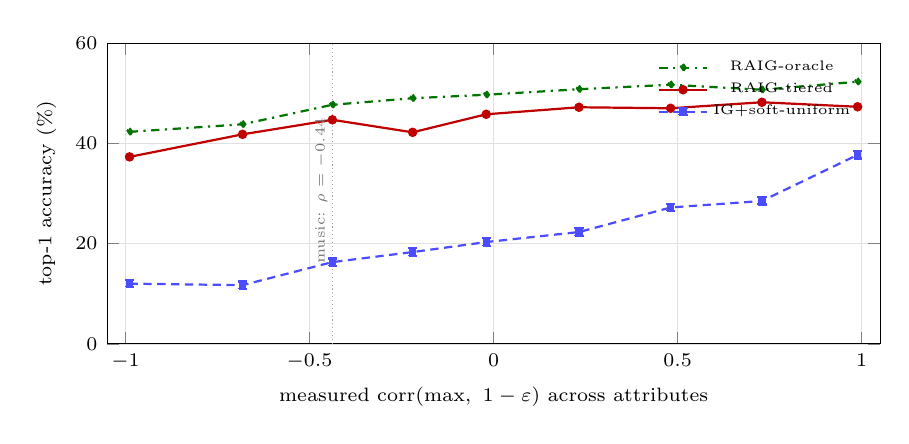
\begin{tikzpicture}
\begin{axis}[
  width=0.94\columnwidth, height=5.4cm,
  xlabel={measured $\mathrm{corr}(\max\Hb,\ 1-\varepsilon)$ across attributes},
  ylabel={top-1 accuracy (\%)},
  xmin=-1.05, xmax=1.05, ymin=0, ymax=60,
  xtick={-1,-0.5,0,0.5,1},
  tick label style={font=\scriptsize}, label style={font=\scriptsize},
  legend style={font=\tiny, at={(0.98,0.98)}, anchor=north east, draw=none,
                fill=none, row sep=-1pt},
  grid=major, grid style={black!12, very thin},
  mark size=1.3pt,
]
\addplot[green!45!black, thick, dashdotted, mark=diamond*] coordinates
  {(-0.989,42.3) (-0.682,43.8) (-0.438,47.7) (-0.220,49.0) (-0.020,49.7)
   (0.232,50.8) (0.481,51.7) (0.729,50.7) (0.989,52.3)};
\addlegendentry{RAIG-oracle}
\addplot[red!75!black, thick, mark=*] coordinates
  {(-0.989,37.3) (-0.682,41.8) (-0.438,44.7) (-0.220,42.2) (-0.020,45.8)
   (0.232,47.2) (0.481,47.0) (0.729,48.2) (0.989,47.3)};
\addlegendentry{RAIG-tiered}
\addplot[blue!70, thick, densely dashed, mark=square*] coordinates
  {(-0.989,12.0) (-0.682,11.7) (-0.438,16.3) (-0.220,18.3) (-0.020,20.3)
   (0.232,22.3) (0.481,27.2) (0.729,28.5) (0.989,37.7)};
\addlegendentry{IG+soft-uniform}
\draw[black!35, thin, densely dotted] (axis cs:-0.438,0) -- (axis cs:-0.438,60);
\node[font=\tiny, anchor=south west, black!55, rotate=90]
  at (axis cs:-0.425,14) {music: $\rho=-0.44$};
\end{axis}
\end{tikzpicture}
\caption{The advantage as a continuous function of the informativeness/
reliability correlation, on a synthetic catalogue family with everything else
held fixed. Classical information gain degrades monotonically as the
correlation turns adversarial, from $37.7\%$ at $\rho=+0.99$ to $12.0\%$ at
$\rho=-0.99$. Reliability-aware selection is close to flat over the same range
($47.3\%$ to $37.3\%$). The correlation therefore measures how badly classical
selection is \emph{harmed}, not whether the correction is \emph{available};
the dotted line marks the correlation measured on the music catalogue.}
\label{fig:rho}
\end{figure}
%----------------------------------------------------------------------

The sweep contains no break-even point. RAIG-tiered leads at every setting,
from $+9.67\pp$ at $\rho = +0.99$---where the informative attributes are also
the reliable ones and there is, on the correlation account, nothing to
correct---to $+30.17\pp$ at $\rho = -0.68$. That is the same lesson the
cross-domain results gave, now on a controlled axis: what the correlation
governs is the \emph{denominator}, how far classical information gain falls,
not whether reliability-aware selection has anything to offer. And the reason
the correction is always available here is the one the previous paragraph
identifies---in this family twelve of the twenty attributes fall in the
reliable tiers and place $76\%$ to $94\%$ of items in a singleton class, so
steering towards them is affordable at every $\rho$.

The practical reading combines the two experiments. A catalogue with an
adversarial correlation \emph{and} an answerable reliable subset is the best
case, and it is where the music catalogue sits. A catalogue with an answerable
reliable subset but no correlation still benefits, and that is dermatology. A
catalogue whose reliable subset cannot identify anything does not benefit
whatever its correlation, and that is mushroom.

\subsection{Abstention}
\label{sec:results-erasure}

Section~\ref{sec:erasure} derives the acquisition function for a user who may
decline to answer, \eqref{eq:erasure}, and attaches a prediction to it: if
abstention correlates with subjectivity in the same direction as error, the two
penalties compound and the bias should be \emph{larger} than the pure-BSC
analysis suggests. Predictions of that kind belong in an experiment rather than
in a future-work list, so we implement the channel and test it. Each attribute
additionally returns an erasure with probability $\delta_f$, tied to its tier
on the reasoning that a user who cannot judge an attribute reliably is also the
one most likely to decline it; an erased turn is consumed but produces no
belief update. Three selectors are compared: classical information gain, blind
to both; RAIG, which models error but not abstention; and RAIG+erasure, which
models both.

\begin{table}[t]
\caption{The abstention channel. Mild is $\delta = (0.02, 0.10, 0.20)$ by tier,
strong is $(0.05, 0.20, 0.40)$; the error channel is heterogeneous
$\lambda = 1.0$ throughout, $n = 450$ paired trials. ``Answered'' is the
fraction of consumed turns that returned an answer rather than an erasure, and
is a consequence of which questions the selector chose.}
\label{tab:erasure}
\centering
\footnotesize
\begin{tabular}{@{}llrrr@{}}
\toprule
\textbf{Abstention} & \textbf{Method} & \textbf{acc.\ (\%)} &
\textbf{answered} & \textbf{subj.\ \%} \\
\midrule
none   & IG+soft-uniform & 2.44 & 1.000 & 53.4 \\
       & RAIG-tiered     & 7.78 & 1.000 & 2.8 \\
       & RAIG+erasure    & 7.78 & 1.000 & 2.8 \\
\midrule
mild   & IG+soft-uniform & 1.56 & 0.849 & 54.3 \\
       & RAIG-tiered     & 5.33 & 0.930 & 1.8 \\
       & RAIG+erasure    & 4.00 & 0.932 & 1.2 \\
\midrule
strong & IG+soft-uniform & 1.11 & 0.692 & 55.6 \\
       & RAIG-tiered     & 4.00 & 0.854 & 1.4 \\
       & RAIG+erasure    & 3.56 & 0.862 & 0.5 \\
\bottomrule
\end{tabular}
\end{table}

Table~\ref{tab:erasure} reports the outcome. There are two results, and the
first is a refutation of our own prediction.

\emph{The absolute advantage shrinks rather than grows.} RAIG-tiered leads
IG+soft-uniform by $+5.33\pp$ with no abstention, $+3.78\pp$ under mild
abstention and $+2.89\pp$ under strong abstention. Measured on the paper's
headline scale, the penalties do not compound; they compress, because
abstention pushes every method towards the floor and there is progressively
less accuracy to win. The prediction of Section~\ref{sec:erasure} is wrong as
stated, and we let it stand in the theory section rather than quietly deleting
it, because the version that survives is worth having: on a \emph{relative}
scale the compounding is real and monotone, with RAIG's accuracy $3.18\times$
IG's without abstention, $3.43\times$ under mild and $3.60\times$ under strong.
The right conclusion is that abstention makes classical selection relatively
worse and absolutely no more distinguishable, which is a weaker claim than the
one we made in advance.

\emph{Modelling abstention explicitly buys nothing here.} RAIG+erasure is
indistinguishable from RAIG-tiered with no abstention (identical, as it must be
when $\delta \equiv 0$) and slightly \emph{worse} under both mild
($-1.33\pp$, $p = 0.24$) and strong ($-0.44\pp$, $p = 0.80$) abstention. Neither
difference is significant, so the finding is an absence rather than a reversal,
but the point estimate is in the wrong direction and the mechanism is
instructive. Because $\delta_f$ is tied to the tier in the same order as
$\varepsilon_f$, the error-based discount has already steered the selector away
from the high-abstention questions: RAIG-tiered gets $93.0\%$ of its turns
answered under mild abstention against classical selection's $84.9\%$, without
modelling abstention at all. The extra $(1-\delta)$ factor then applies a
second discount to attributes that are already being avoided, driving the
subjective share of questions to $0.5\%$ at strong abstention and narrowing the
question pool towards the reliable-subset ceiling of
Section~\ref{sec:results-synthetic}---the same over-correction that produces
the clean-condition collapse.

The practical implication is that a deployed system facing abstention should
model it in the \emph{belief update}, where an erasure must not be treated as
evidence, and can safely leave the selector to the error term alone---provided
abstention and error are ordered the same way across attributes. Where they
are not, \eqref{eq:erasure} is the correct criterion and this experiment says
nothing against it.

\subsection{Correlated Answer Errors}
\label{sec:results-correlated}

The channel of Section~\ref{sec:method} draws every answer independently at
rate $\varepsilon$. A real listener who misjudges ``is it energetic?'' is
likely to misjudge it the same way when asked again, so independence is the
modelling assumption most likely to be flattering to us, and it should be
attacked directly rather than listed as a limitation.

We attack it with a deliberately harsh alternative. The first time a
\emph{subjective} attribute is answered wrongly in a session, that attribute is
marked corrupted for the remainder of the session and every later question
about it is forced wrong; objective and semi-objective attributes keep
independent draws, since simple slips rather than conceptual confusion are the
plausible failure there. This turns a rate-$\varepsilon$ channel into a
per-session absorbing one on exactly the attributes classical selection
prefers. Both variants run inside the same loop and consume the same random
stream in the same order, so the independent and correlated columns are paired
trial for trial and any difference between them is the correlation and nothing
else.

The result, in Table~\ref{tab:correlated}, strengthens rather than weakens the
paper's conclusion.

\begin{table}[t]
\caption{Independent against correlated answer errors, heterogeneous
$\lambda = 1.0$, $n = 900$, paired trial for trial across all four cells.
Correlating errors on subjective attributes costs classical selection
$0.78\pp$ and costs reliability-aware selection exactly nothing.}
\label{tab:correlated}
\centering
\footnotesize
\begin{tabular}{@{}lrrr@{}}
\toprule
\textbf{Method} & \textbf{independent} & \textbf{correlated} &
\textbf{difference} \\
\midrule
IG+soft-uniform & 2.78 & 2.00 & $-0.78\pp$ ($p = 0.016$) \\
RAIG-tiered     & 7.78 & 7.78 & $+0.00\pp$ ($p = 1.00$) \\
\midrule
$\Delta$ (RAIG $-$ IG) & $+5.00\pp$ & $+5.78\pp$ & \\
McNemar $p$ & $3.6\times10^{-7}$ & $3.1\times10^{-9}$ & \\
\bottomrule
\end{tabular}
\end{table}

Correlating the errors costs IG+soft-uniform $0.78\pp$---seven trials that it
won under independent errors and loses under correlated ones, and not a single
trial in the other direction---while RAIG-tiered's outcome is
\emph{bitwise identical} across the two variants: zero discordant pairs out of
$900$. The paired advantage therefore grows from $+5.00\pp$ to $+5.78\pp$, and
its $p$-value improves by two orders of magnitude.

The asymmetry is not luck, and it follows from Table~\ref{tab:asked}. The
absorbing mechanism can only fire on subjective attributes. Classical selection
spends $53.9\%$ of its budget there and is exposed to it on most turns;
RAIG-tiered spends $2.9\%$ and is almost never exposed, and in these $900$
sessions it was never exposed twice to the same subjective attribute, which is
what a repeat requires. A selector that avoids the attributes on which users
are unreliable is, as a side effect, also robust to their errors being
persistent rather than fresh---which is a property worth having, since
persistence is the more realistic model and the harder one to estimate.

We do not claim this exhausts the question. Errors could correlate
\emph{across} attributes rather than within one---a listener with an unusual
notion of ``energetic'' probably also has an unusual notion of
``danceable''---and that structure would penalise any method that clusters its
questions within a tier, including ours. Testing it would require a
user-level latent-trait model that we do not have data to fit.

\subsection{An Online Alternative to the Tiers, and Its Catalogue-Size Dependence}
\label{sec:results-streaming}

Section~\ref{sec:results-em} removes the three assumed tier values by learning
a crossover vector \emph{offline}, from six hundred already-completed
sessions, before the vector is ever used. A natural sharper version of the
same idea is to skip the offline pass entirely: re-estimate the per-attribute
crossover \emph{online}, from the trials the deployed system is already
running, with no tier annotation assumed even as a cold-start value. We built
and tested exactly this variant, \textbf{RAIG-streaming}, and report both what
happened and why, because the failure is as informative as a success would
have been.

\emph{The mechanism.} Every attribute starts at a single neutral crossover,
$\hat\varepsilon = 0.10$, no tiers involved. Between batches of paired
trials---not inside the per-turn loop itself, which would couple the estimate
to a single session's own noise---the same attribute-pooled
expected-disagreement statistic Section~\ref{sec:results-em} computes offline
is folded into a running per-attribute total, and the estimate used by the
NEXT batch is the resulting mean, shrunk toward the neutral prior with a
pseudo-count of sixty so that an attribute with little evidence cannot swing
on a handful of noisy readings. A fraction of turns, $20\%$, is forced to a
uniformly random available question regardless of the current estimate,
mirroring the forced-exploration fix Section~\ref{sec:results-em}'s offline
estimator already needed for the identical reason.

\emph{On the full catalogue, it loses, to a diagnosed mechanism rather than to
noise.} At the primary condition and $T=70$ (Table~\ref{tab:streaming}),
RAIG-streaming reaches $18.56\%$ against RAIG-tiered's $38.56\%$---a
$20.00\pp$ deficit, exact McNemar $p = 5.0\times10^{-27}$---and even trails
plain classical information gain's $27.11\%$ by $8.56\pp$
($p = 4.4\times10^{-6}$). The cause is a feedback loop the fixed tiers cannot
experience because they never move. \texttt{genre} alone compiles to $113$ of
the catalogue's $193$ questions and is genuinely the most reliable attribute
in it; the moment the running estimate correctly notices this, the selector
asks it more, which supplies more evidence for exactly that attribute and
none for the other nineteen, whose own estimates stay noisy and drift toward
the unreliable end of the clip range from thin, badly-timed samples. Measured
directly over these $900$ sessions, \texttt{genre} takes $58.6\%$ of every
question RAIG-streaming asks, against $36.0\%$ for the curator's fixed tiers
and $24.6\%$ for classical information gain at the same operating
point---a share no fixed annotation ever produces, because a fixed annotation
cannot compound the way a live one can. An earlier, unregularised attempt
(no shrinkage, $10\%$ exploration) put \texttt{genre}'s share at $78.7\%$ and
reached only $5.9\%$ accuracy; the shrinkage-and-exploration fix reported here
roughly triples that, but does not close the gap to the tiers at this scale.

\begin{table}[t]
\caption{Static tiers against the online alternative, primary condition,
$T=70$, $n=900$. $\Delta$ and $p$ are against RAIG-tiered, exact McNemar,
Holm-corrected within this family.}
\label{tab:streaming}
\centering
\footnotesize
\begin{tabular}{@{}lrrr@{}}
\toprule
\textbf{Method} & \textbf{top-1 (\%)} & \textbf{$\Delta$ (pp)} & \textbf{$p$ (Holm)} \\
\midrule
IG+soft-uniform            & 27.11 & $-11.44$ & $5.1\times10^{-9}$  \\
RAIG-streaming             & 18.56 & $-20.00$ & $5.0\times10^{-27}$ \\
RAIG-streaming+stop@0.5    & 19.78 & $-18.78$ & $5.2\times10^{-24}$ \\
RAIG-streaming+stop@0.7    & 18.00 & $-20.56$ & $1.2\times10^{-28}$ \\
RAIG-streaming+stop@0.9    & 17.78 & $-20.78$ & $1.2\times10^{-28}$ \\
\textbf{RAIG-tiered}       & \textbf{38.56} & --- & --- \\
\bottomrule
\end{tabular}
\end{table}

\emph{Raising the cap alone, on the tiers, is the clean win in this
experiment.} RAIG-tiered itself improves from $26.56\%$ at the budget of
Table~\ref{tab:primary} to $38.56\%$ simply by raising $T$ from $40$ to $70$
with nothing else changed---an operating-point change, not a methodological
one, and the only unambiguous gain reported in this subsection.

\emph{Early stopping at $T=70$ behaves exactly as
Section~\ref{sec:results-behaviour} predicts it will at $T=20$: it mostly
does not fire.} A confidence threshold of $0.90$ crosses in $1.1\%$ of
RAIG-streaming sessions by turn seventy; $0.70$ in $2.0\%$; $0.50$ in $3.6\%$.
None of the three changes accuracy by a significant amount relative to
running the streaming estimator to completion (Table~\ref{tab:streaming}, all
$p_{\text{Holm}} = 1.00$). Forty additional questions past the entropy floor
still mostly does not buy the confidence a stopping rule needs to act on; it
buys accuracy at a fixed budget instead, which is the mechanism
Table~\ref{tab:streaming} already reports.

\emph{The deficit is not fixed: it is catalogue-size dependent.}
Section~\ref{sec:results-size} already reports that the RAIG-over-IG
advantage survives at every catalogue size tested. We repeated the
online-versus-static comparison specifically, on an independently drawn
$5{,}000$-item subset (identifiability ceiling $99.5\%$, floor $12.28$ bits)
with the budget extended to $T=200$ (Table~\ref{tab:streamsize}). The pattern
reverses: by $T=80$ the two are statistically indistinguishable ($71.00\%$
against $71.44\%$, $p = 0.85$), and the gap stays indistinguishable from zero
through $T=200$ ($73.89\%$ against $72.67\%$, $p = 0.52$)---RAIG-streaming's
point estimate is even fractionally higher at the longest budget tested, but
not significantly so. We do not claim the online estimator wins at small
scale; we report that the deficit it shows at full scale is not a fixed
property of the method, and that a smaller identification task gives the
same online estimator enough of its own budget to reach parity with an
annotation it was never given.

\begin{table}[t]
\caption{The online estimator against static tiers on a $5{,}000$-item
subset, one independent draw, $n=900$, primary condition. $p$ is the exact
McNemar test between RAIG-streaming and RAIG-tiered at that column.}
\label{tab:streamsize}
\centering
\footnotesize
\begin{tabular}{@{}lrrrrr@{}}
\toprule
\textbf{Method} & \textbf{$T{=}40$} & \textbf{$T{=}60$} & \textbf{$T{=}80$} &
\textbf{$T{=}100$} & \textbf{$T{=}200$} \\
\midrule
IG+soft-uniform  & 41.33 & 56.67 & 58.44 & 58.44 & 58.00 \\
RAIG-tiered      & 61.33 & 69.56 & 71.44 & 72.89 & 72.67 \\
RAIG-streaming   & 47.89 & 64.89 & 71.00 & 72.11 & 73.89 \\
\midrule
$p$ (streaming vs.\ tiered) & --- & --- & $0.85$ & $0.71$ & $0.52$ \\
\bottomrule
\end{tabular}
\end{table}

\emph{Reading the two results together.} What the online estimator lacks
relative to the offline one of Section~\ref{sec:results-em} is repetition:
the offline estimator replays the same fixed logged sequence eight times,
each pass recomputing belief under a better crossover guess; the online one
sees every trial once, under whichever guess happened to be current when
that trial ran. On a catalogue small enough, or a budget long enough, that a
single pass supplies adequate coverage of every attribute, this costs little.
On the full catalogue at $T=70$ it costs a great deal, because
\texttt{genre}'s dominance of the question pool gives the feedback loop room
to run before the other nineteen attributes accumulate enough evidence to
compete. We report this as a diagnosed limitation with a concrete next
step---an online estimator that replays its own most recent batch a small,
fixed number of times before committing to the next one, borrowing the
offline estimator's repetition without its six-hundred-session
latency---rather than as a closed question.
